\documentclass[]{final_report}
\usepackage{graphicx}
\usepackage{hyperref}


%%%%%%%%%%%%%%%%%%%%%%
%%% Input project details
\def\studentname{Colin Smith}
\def\projecttitle{Using RFID to Remember}
\def\supervisorname{Lorcan Coyle, Aaron Quigley}
\def\moderatorname{Fintan Costello}


\begin{document}

\maketitle
\tableofcontents\pdfbookmark[0]{Table of Contents}{toc}\newpage

%%%%%%%%%%%%%%%%%%%%%%
%%% Your Abstract here

\begin{abstract}

\textbf{\textsl{RFID has proved to be a useful technology, becoming more common with development of
applications to benefit people in everyday useful ways. This
project proposes to use this technology to aid human memory, and specifically to
help people find lost items. For most people, losing a wallet or a mobile phone is a common
occurrence and could benefit from such a system. Using the system is simple, it consists of an RFID component which identifies user interactions with objects. This data is used to help people locate lost items through interacting with a lost and
found application, which is based on human readable cues. For example, `The
user last took their wallet out of their bag at 12:00 along with their car keys'.
The cues are constructed based on interactions with such objects, augmented with location data, and interactions with other people. Users interact with these cues through a
web page and also receive alerts on potentially lost items, through a built in system display.}}


\end{abstract}
\newpage

%%%%%%%%%%%%%%%%%%%%%%
%%% Acknowledgments

\chapter*{Acknowledgments}

In your Acknowledgments section, give credit to all the people who helped you in your project.

%%%%%%%%%%%%%%%%%%%%%%
%%% Introduction

\chapter{Introduction}
The goal of this project is to build a system which helps users to find lost items, such as a phone or wallet. It is based on RFID technology, which is used to record user interactions with these items. RFID is a way of wirelessly identifying objects, consisting of a reader and tags. When an item is tagged, it can be uniquely identified when it comes into range of the reader. Using these records of user interactions with objects, an Aide Memoire can be developed. This will take the form of a web site where users can obtain information about their interactions with a lost item, and aid them in remembering where they may have lost it. The data gathered using RFID tags is supplemented using Bluetooth technology. Bluetooth enables the system to wirelessly identify people based upon their mobile phone Bluetooth ID, and to identify locations based on static Bluetooth nodes.  

The system is made up of a mobile component and a website. The mobile component consists of the RFID reader connected to a portable micro-computer, which has built in Bluetooth capabilities. This will gather information about the users' interactions such as when they had certain items and what locations and people they have come in contact with. The static component consists of a server and lost and found website. The data gathered by the micro-computer is wirelessly
transmitted to the server, stored in a database, and presented to the
user through the website. 

This report presents a detailed overview of the goals, design and outcome of the system implementation. It includes a full description of the systems design and construction leading to system evaluations and conclusions. Chapter~\ref{background} discusses background research relevant to the project. The papers presented are relevant to the technologies being used and provide useful insight into related fields of research involving these technologies. The background research also gives further insight into the applicability or usefulness of RFID for the proposed system design, and explores the concepts and goals of this project. Chapter~\ref{implementation} gives a detailed description of the system's implementation. This includes the system's design with regards to the hardware being used and the systems form factor. This chapter also includes descriptions of the system's data processing techniques and overviews of the software technologies being used. Chapter~\ref{evaluations} describes how the system is evaluated and tested. This includes the results of these tests and the conclusions which can be drawn from them. Chapter~\ref{future} presents the final conclusions of this work based upon the overall evaluations and performance of the system. The applicability of this system for its intended purpose are discussed and the future research potential for this technology is explored. 

The following is the original specification for this project:

Title: Using RFID to Remember

Lecturer: Lorcan Coyle and Aaron Quigley

Description: Associating interactions between users and artefacts in their everyday surroundings could be a useful way of helping people remember where they left them. When people cannot find something, simple cues like `you left your keys on the dresser table', or `i saw you take your wallet with your mobile phone' are naturally helpful. This project seeks to record a person's interactions with everyday items and generate useful cues to the user when they lose something.

This project builds on an earlier ODCSSS summer school project, where an RFID reader is embedded in a glove and RFID tags are attached to kitchen implements. The reader can see when the user interacts with any item that has an attached tag and know what that item is. 

The earlier project recorded interactions with the kitchen implements and used them to detect when the user was completing a routine task (e.g., making a cup of tea). This project would have access to the outputs of that project and one of the challenges of this project would be to understand, reuse, and extend the earlier work.

Mandatory: Software must be built to recognise a human user's interactions with everyday objects. These objects would be attached with RFID tags and the user will interact with them using the rfid glove.

The software must be capable of giving useful (if simple) cues to remind the user where lost items are, e.g. `you interacted with your mobile phone at 2:01pm, 32 seconds after you interacted with your car keys and 21 seconds before you interacted with your wallet'

Discretionary: A useful way for the software to communicate with the user should be developed - this might be through a lost-and-found web page, or a display attached to the glove.

Exceptional: More complex, human readable cues should be developed, e.g., `you last had your mobile just after 2pm; you were also using your car keys and wallet at that time'.

\chapter{ Background Research}
\label{background}

\section{Introduction}

This chapter presents an overview of background research relevant to the project. The research papers discuss a number of relevant concepts such as ubiquitous computing and wearable technology. These papers give a positive insight into different implementations of the proposed technologies, leading to some important conclusions on the application of RFID technology in this project.

\subsection{An Introduction to RFID Technology}

RFID is a technique for wirelessly identifying objects, which has become increasingly recognised for its many potential mainstream applications and uses. There are various types of RFID available, suited to different types applications. From the highest level RFID can be divided into two classes, active and passive~\cite{intel}. Active RFID requires each individual tag to have its own built in power supply. Passive RFID does not use self powered tags, they are instead charged by the reader using magnetic induction. The system being implemented for this project is based on passive RFID. Active tags would require future maintenance, such as battery replacement, and are impractical for the projects concepts. Active tags are also significantly larger and heavier. Passive tags can be as small as a one euro coin, making them ideal for placing on objects. Using the passive technique the reader can power the tags and allow them to transmit a signal corresponding to its unique ID \cite{intel}. Figure~\ref{fig:readertag} shows the RFID reader used in this system and an example tag. 

\subsubsection{2.1.1.2 Passive RFID}
The RFID method used in this system is known as passive RFID \cite{intel}. This is opposed to active RFID where the tags contain their own power source. As these tags are much larger and will eventually require maintenance such as battery replacement passive RFID is the ideal choice. In this technique tags are powered by the reader using a method known as electromagnetic induction, essentially building a charge from the readers magnetic field. Once powered the tag can transmit its unique hexadecimal ID. Passive RFID tags are much smaller which makes them ideal for placing them on common items. They are unobtrusive and could, for example, be placed inside the battery cover of a phone. This is consistent with the goals of ubiquitous computing and the project where useful technology can blend naturally into our environment \cite{weiser}. 

\begin{figure}[h]
\centering
\fboxsep 1mm
\framebox{
	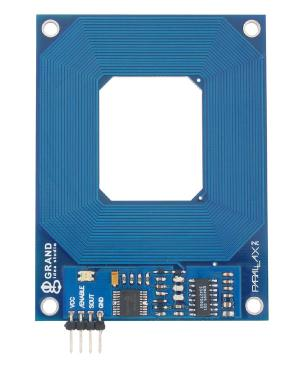
\includegraphics[width=3cm, height=4cm]{reader} 
	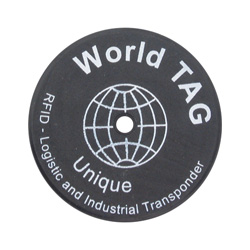
\includegraphics[width=3cm, height=3cm]{tag}
}
\caption{RFID reader and Tag \cite{parallax}}
\label{fig:readertag}
\end{figure} 

\subsection{The Computer for the 21st Century}

Mark Weiser's seminal paper on ubiquitous computing proposes the concept of `embodied virtuality'~\cite{weiser}. He describes how in today's world information is everywhere in our environment, so much so that we do not even notice it. Technology is also a common element in our environment but it has yet to reach its full potential. He conceives a system in which computers cover free surface spaces in our surroundings, connected through an invisible network, and become part of our normal environment. One is surrounded by technology, but it vanishes into the background so as its presence is not even noted. Such a system has countless applications. This is similar to the ideas of Dey et al. \cite{dey} in which the concept of technology integrating and blended seamlessly into our environment is explored. Weiser's proposed system identifies people through badges, for example, and adjusts the environment based on the individual. A person enters a room and their calls and messages are automatically transferred to them through the environment. When a person enters their place of work they are identified, at which point their office logs them in and displays documents and files, or perhaps starts to make coffee, before they have even arrived.  An important point the author raises is that such complex systems do not require the use of complex artificial intelligence techniques. All these systems can simply be derived from knowing basic information about a persons' activities \cite{weiser}. This project proposes a similar concept. From knowing simple information about a users' interactions with objects, a more complex and useful application can be derived. 

\subsection{Chatchayanuson's Kitchen Tracker}

Chatchayanuson et al.'s Kitchen Tracker system proposes to aid people with grocery shopping~\cite{ece}. The system consists of stationary RFID readers in a kitchen and tags placed on key grocery items within it. As items are removed from the kitchen, i.e., used or thrown away, the RFID readers are used to identify these items. This data is used to assist in grocery shopping indicating key items that are needed in the kitchen through real time synchronisation with a phone or PDA. These implementations are based on smart home concepts \cite{ece}. The system is an integrated and useful system contained within a home environment, assisting in every day tasks without being obtrusive to a person's life. An important point raised by this implementation is that such technologies should be unobtrusive and blend naturally into our environment. 

\subsection {Ubiquitous Memories}

Kawamura et al.'s Ubiquitous Memories is an innovative system designed to augment human memory through interaction with objects, and explores the area of wearable computing \cite{ubi}. From a hardware perspective the system consists of a head mounted display over the left eye for displaying video to the user. This eyepiece also incorporates a camera to record user�s activities and experiences. There is an RFID reader on one wrist to read tagged objects. These are both connected to a remote control for the system which connects to a hip-mounted wearable computer. This is shown in figure~\ref{fig:borg}. This computer connects wirelessly to a LAN.
The system records the user�s experiences and activities and passes them to a server to be stored in a video database. Objects related to specific events are RFID tagged. When a tag is read the system replays a video related to that object, mimicking the behavior of human memory. When people touch objects they often recall associated memories \cite{ubi}. The system was tested using memory and recall techniques using different memory aids, one of which being the Ubiquitous Memories system. This determines the effectiveness of the system in aiding human memory and also offers insight into alternative ways of achieving this. The system is compared to other methods, in this case memory recall techniques that don't involve technology. Instead of simply rating the system performance based solely on testing it for what it is designed for, it is compared to these other methods which are designed to achieve the same goal. This knowledge could be potentially used to refine or augment the system in the future. It is this authors opinion that, like the kitchen tracker system and Weiser's concepts \cite{ece, weiser}, it is important to point out that such a system needs to be unobtrusive and feel natural in our environment. This is particularly relevant for wearable computing in which the user is often in direct physical contact or in possession of the technology while they undertake everyday tasks.  

\begin{figure}[h]
\centering
\fboxsep 2mm
\framebox{
	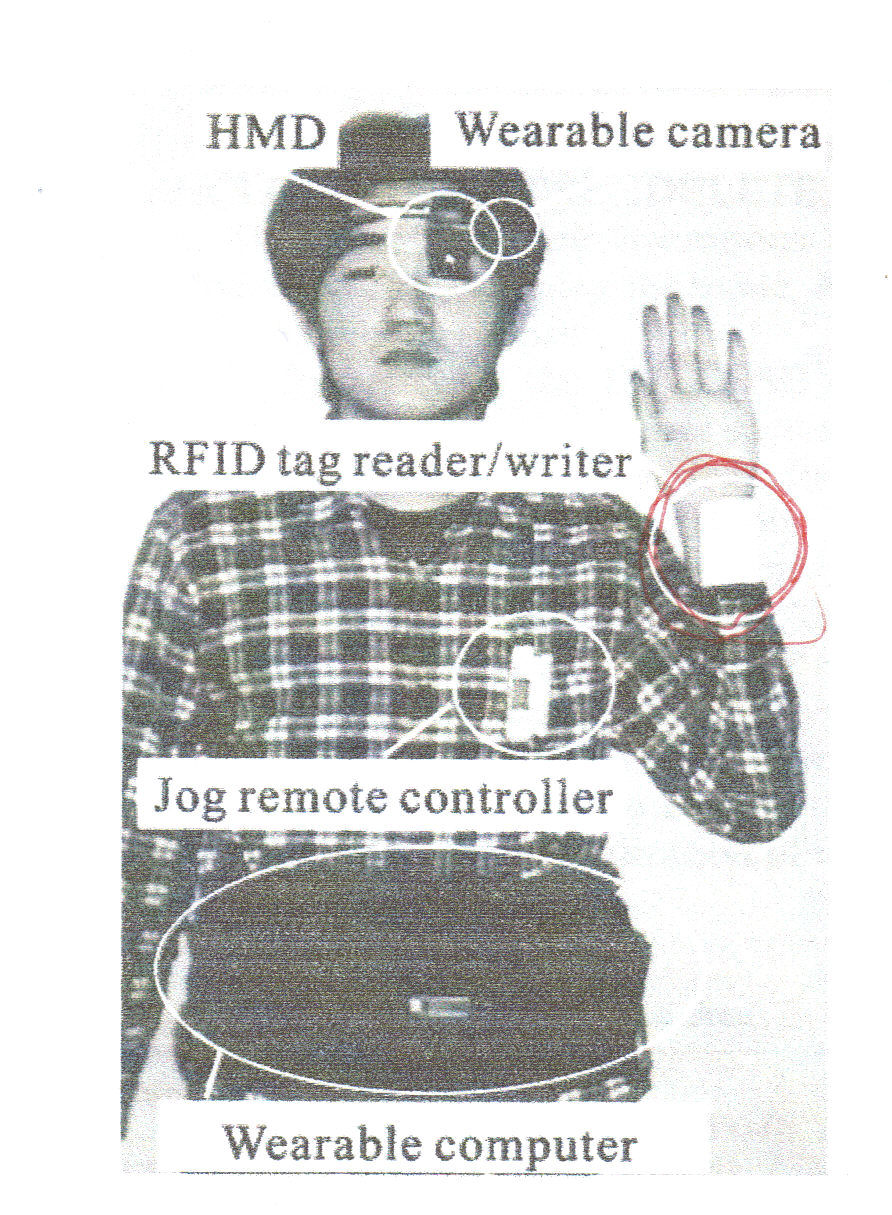
\includegraphics[width=4cm, height=6cm]{borg}
}
\caption{`Ubiquitous Memories' system \cite{ubi}}
\label{fig:borg}
\end{figure} 

\subsection {Schmidt and Gellersen's RFID glove}

Like the Ubiquitous Memories system, Schmidt and Gellersen's RFID glove explores the area of wearable computing \cite{ubi, schmidt} . In this area there is often difficulty in providing computer input if systems carry high cognitive loads or
performance problems in their deployment. They explore human computer interaction using an RFID based system in an attempt to overcome the inherent shortcomings of wearable computing. The main concept is based on implicit human
computer interaction. Implicit interaction is described as actions which are not primarily
intended to be used as computer input but can still be used as such in some useful way. This is very relevant in this proposed project and similar to weiser's concepts \cite{weiser}, where computer inputs will be used to create a useful application. Their
implementation consists of a glove with an integrated RFID reader. The reader is connected
through a serial connection to a wearable computer. RFID tag IDs are mapped to a specific
URL which increases a counter each time a tag is read. They conclude that such an implementation
effectively overcomes the traditional problems associated with user input in wearable
computing, and propose that such a system would form a sound base for implementing
practical applications of the technology~\cite{schmidt}. Their work indicates how RFID can overcome high cognitive loads which are typical of wearable technology, where the technology does not require a user's attention or interaction in order to gather useful computer input and data.  

\begin{figure}[h]
\centering
\fboxsep 2mm
\framebox{
	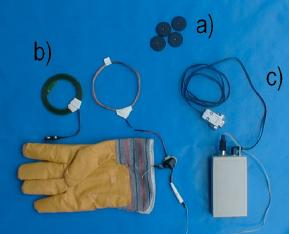
\includegraphics[width=5cm, height=4cm]{schmidt}
}
\caption{RFID glove components: a) RFID Tags, b) Reader Coils,
c) Wearable Tag Reader \cite{schmidt}}
\label{fig:scmidt}
\end{figure} 

\subsection {Intel's iGlove}

In building useful applications with RFID technology a technique is required in order to allow
the computer to correctly interpret its inputs. Intel Seattle's iGlove research project explored the concept of recognising and interpreting an individuals activities from large sets of possibly related RFID readings \cite{intel2}. Like Schmidt and Gellersen, their system prototype was an RFID enabled glove with the antenna located in the palm. This is connected to a reader with radio capabilities for communicating with a computer. The glove components are all housed
in a plastic box on the outer side of the glove, which overall makes the system compact and
unobtrusive, which can be seen in figure \ref{fig:iglove}.

One difficulty their system faced was interpreting `variety', for example the same task could be completed in different ways or in a different order of steps. This would give various combinations of data inputs leading to the difficulty of interpreting them correctly. The proposed solution was to represent tasks in a sequence, or probable sequence, of the objects used, which resulted in a high level of system accuracy and performance. This is shown by their systems ability to correctly identify various tasks being undertaken by the user \cite{intel2}. This project's proposed system will also gather large amounts of data which and similarly to this project may present inherant difficulties in interpreting it correctly, which will need consideration in the systems data processing techniques. 

\begin{figure}[h]
\centering
\fboxsep 1mm
\framebox{
	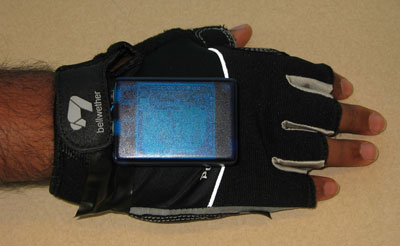
\includegraphics[width=6cm, height=4cm]{iglove} 
	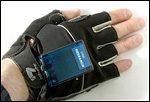
\includegraphics[width=6cm, height=4cm]{iglove2}
}
\caption{Intel's `iGlove`}
\label{fig:iglove}
\end{figure} 

\subsection {Lustig's RFID glove}

Lustig and Coyle developed a similar RFID glove system following intel's work on the iGlove \cite{intel2}, designed to identify
specific tasks carried out by a user \cite{cait}. A glove design was implemented with an RFID reader built into the palm, as shown in figure \ref{fig:lustig}. This was connected to a micro-computer with wireless capabilities. The micro-computer can connect wirelessly to a server which in turn can update a database of tag reads and pass this information to a web page. The system is designed to recognise individual tasks by associating each one with a number of relevant tags. This project extends this research building upon the work already achieved while focusing on a related but different goal.  Although this project utilised some similar technologies, such as an RFID reader and micro-computer, the proposed project is a very different implementation and different application, the lost and found system. It will utilise more data inputs via Bluetooth technology, and more advanced user interaction, achieved through an LCD display. Having said this it has proven useful to take into account the results and findings of their work. It was found that a glove implementation was considerably restrictive to the user, which does not conform to the principles of ubiquitous and wearable computing, which are some of the main goals of this project. This was considered a strong motivation for a new proposed form factor. 

\begin{figure}[h]
\centering
\fboxsep 2mm
\framebox{
	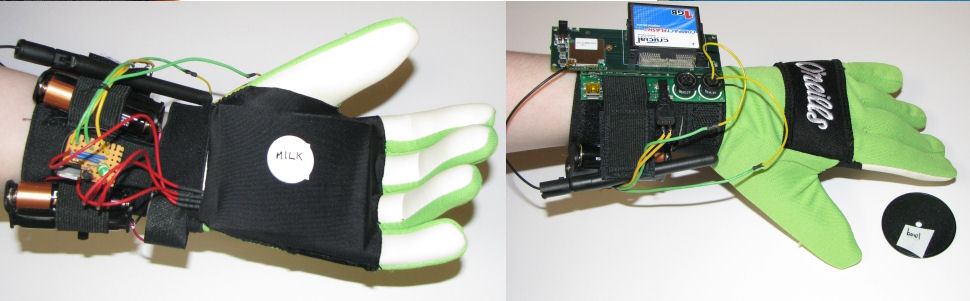
\includegraphics[width=15cm, height=4cm]{lustig}
}
\caption{Lustig and Coyle's RFID glove}
\label{fig:lustig}
\end{figure} 

\subsection{Activity Recognition}

Logan et al. explored the abilities of different sensing equipment \cite{beth}. This research involved the use of intel's previous research on the iGlove and their later work on the iBracelet \cite{intel2, intel3}. The test system was based on a house equipped with over 900 sensor inputs, such as RFID tags, current and water flow sensors, and infrared motion detectors. The concept is also similar Lustig and Coyle's RFID glove, in that it uses sensor input to recognise human interactions and activities in a home environment \cite{cait}. In this evaluation the effectiveness of the sensor types is discussed. In the case of RFID, the user was equipped with an RFID bracelet for reading tags in the environment, sending tag reads wirelessly to a database. The results of the experiment showed that RFID performed quite poorly. It was found that this was due to the reader detecting very few of the objects being touched. There were various reasons for this, such as opposite hands being used to interact with objects, and temporary removal of the bracelet for hygiene reasons. This raises a conflicting point to the other implementations, that RFID may not necessarily be useful in some instances. For example if a person is washing dishes they cannot have electronic equipment attached to their hands \cite{beth}.    

\subsection{Recognising Assembly Tasks}

Ward et al. explored the concept of activity recognition and ubiquitous computing \cite{jamie}. Mobile workers, such as maintenance personnel, often face difficulties in accessing useful information relevant to their task. For example a person may need to access a PDA to bring up schematics which requires complete physical and mental attention. The proposed concept involves identifying users' activities and automatically displaying task relevant data through a head mounted display. This involves both sound and accelerometer sensors, for gesture identification, to gather data and use different algorithmic methods to identify individual tasks. The arm mounted sensors are shown in figure \ref{fig:assembly}. One problem with this, similar to that of Logan et al., involves non relevant activities \cite{beth}. For example, while a user undertakes a task they may momentarily break from this, perhaps to take something from their pocket. Their system was tested on a `mock' scenario where a user constructs a simple item from wood. Although their results were promising they conclude that their approach would be more applicable in a home environment, especially with regards to sound identification. They propose to explore other sensor and algorithmic methods, one of which being RFID, to improve the performance of the system~\cite{jamie}.

\begin{figure}[h]
\centering
\fboxsep 2mm
\framebox{
	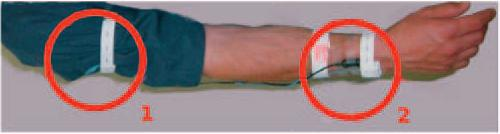
\includegraphics[width=10cm, height=3cm]{worker}
}
\caption{Arm mounted microphones and accelerometers}
\label{fig:assembly}
\end{figure}      

\section{Conclusions}
Much of this previous work in RFID applications offers some important guidance and insight for this project.
One important point raised by many of the discussed research papers is that such systems need to be
unobtrusive, feel natural to a user, and blend naturally into our environment. Ubiquitous
Memories and Chatchayanuson et al.'s kitchen tracker are good examples of this, as well as the important concept of ubiquitous computing \cite{ece, ubi}. Weiser raises another important point which is relevant to this project's system. From simply knowing some basic information, such as where you where at certain time, a more complicated and useful application can be derived, in this case a memory aid \cite{weiser}.

There are often many problems facing the concept of �wearable computing� systems, as discussed by Schmidt and
Gellerson, such as problems with performance. While this is true, it is suggested RFID offers
a sound base for implementing practical applications of these technologies and overcoming
such associated problems \cite{schmidt}. In conflict to this, Logan et al. suggested that RFID may not be useful in some instances, however their evaluation involved recognition of many, very complex user activities, over a long period of time \cite{beth}. In the instances of low performance involving RFID it seems, in this author's opinion, that the reasons for this could have been taken into account or avoided through revising and augmenting activity recognition and sensor techniques of the system. The application in this case is also quite different to that of this proposed project. Identifying a large number of complex tasks as a user undertakes their everyday home activities involves a high number of random factors, such as spontaneously switching between tasks. In the proposed system items will be static in a certain sense, where an item is placed in a pocket within very close proximity to the reader. The possibility of not reading an item in this form factor is extremely low, as discussed in section~\ref{testresults}. It can be concluded that with this systems form factor and design, RFID technology will prove very effective. 

Lustig and Coyle found their RFID system to be very restrictive \cite{cait}. This project will explore an alternative form factor in order to overcome these disadvantages. This project will use some of the proven hardware and technologies as Lustig and Coyle's earlier work, such as the micro-computer and RFID reader, but with a different implementation and application. Their system followed the work of Intel in using RFID to identify user's activities, whereas this project proposes to gather data on a user's interactions with objects. It will also take into account more useful information, such as location and interactions with other people. Interaction between user's and the system will augmented using a built in LCD screen to display relevant information.  

\chapter{System Implementation}
\label{implementation}

\section{Introduction}
This chapter presents a detailed overview of the systems design. This includes the systems form factor and the types of hardware used. The system's data processing techniques are discussed with descriptions of how data is gathered, stored, and used in the application.   

\section{System Form Factor}
The initial concept and form factor of the system was an RFID enabled glove, inspired by the work of Lustig and Coyle~\cite{cait}. The major downfall of their system was the inherent restrictiveness of the glove's design. Also their system was based upon a very different application, recognising user activities, and utilised some similar technologies. It is also the opinion of this author that an RFID enabled glove design is very obtrusive to a users everyday activities, and is not consistent with the ideals of technology blending naturally into our environment. For these reasons a different system form factor is proposed. A box was designed using a 3D printer to house the mini computer. This box along with the RFID reader are held within a small pouch. This pouch can be carried easily within a pocket or a bag. The initial concern with this design is the limited range of the RFID reader, however due to the limited capacity of pockets and bags the reader will be constantly in close proximity to tagged items. This is discussed further in chapter~\ref{evaluations}.  

[Insert picture of pouch when its made. N.B: Learn to sew]

\section{Hardware Design}
There are a number of key components required in this project. The mobile component of the system consists of an RFID reader connected to a Gumstix computer. The Gumstix is a mini computer running a Linux operating system~\footnote{Gumstix information can be found here: www.gumstix.com}. To facilitate the functionality of the system, the Gumstix is expanded with wireless capabilities, two serial connections, and has an integrated Bluetooth module. To connect the reader to the Gumstix a small circuit is constructed which regulates a 5v power supply for the reader and relays tag reads to the Gumstix through one of the serial ports. Figure~\ref{fig:circuit} shows the RFID reader connected to the Gumstix. 

\begin{figure}[h]
\centering
\fboxsep 1mm
\framebox{
	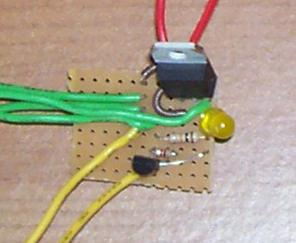
\includegraphics[width=6cm, height=6cm]{circuitShot} 
	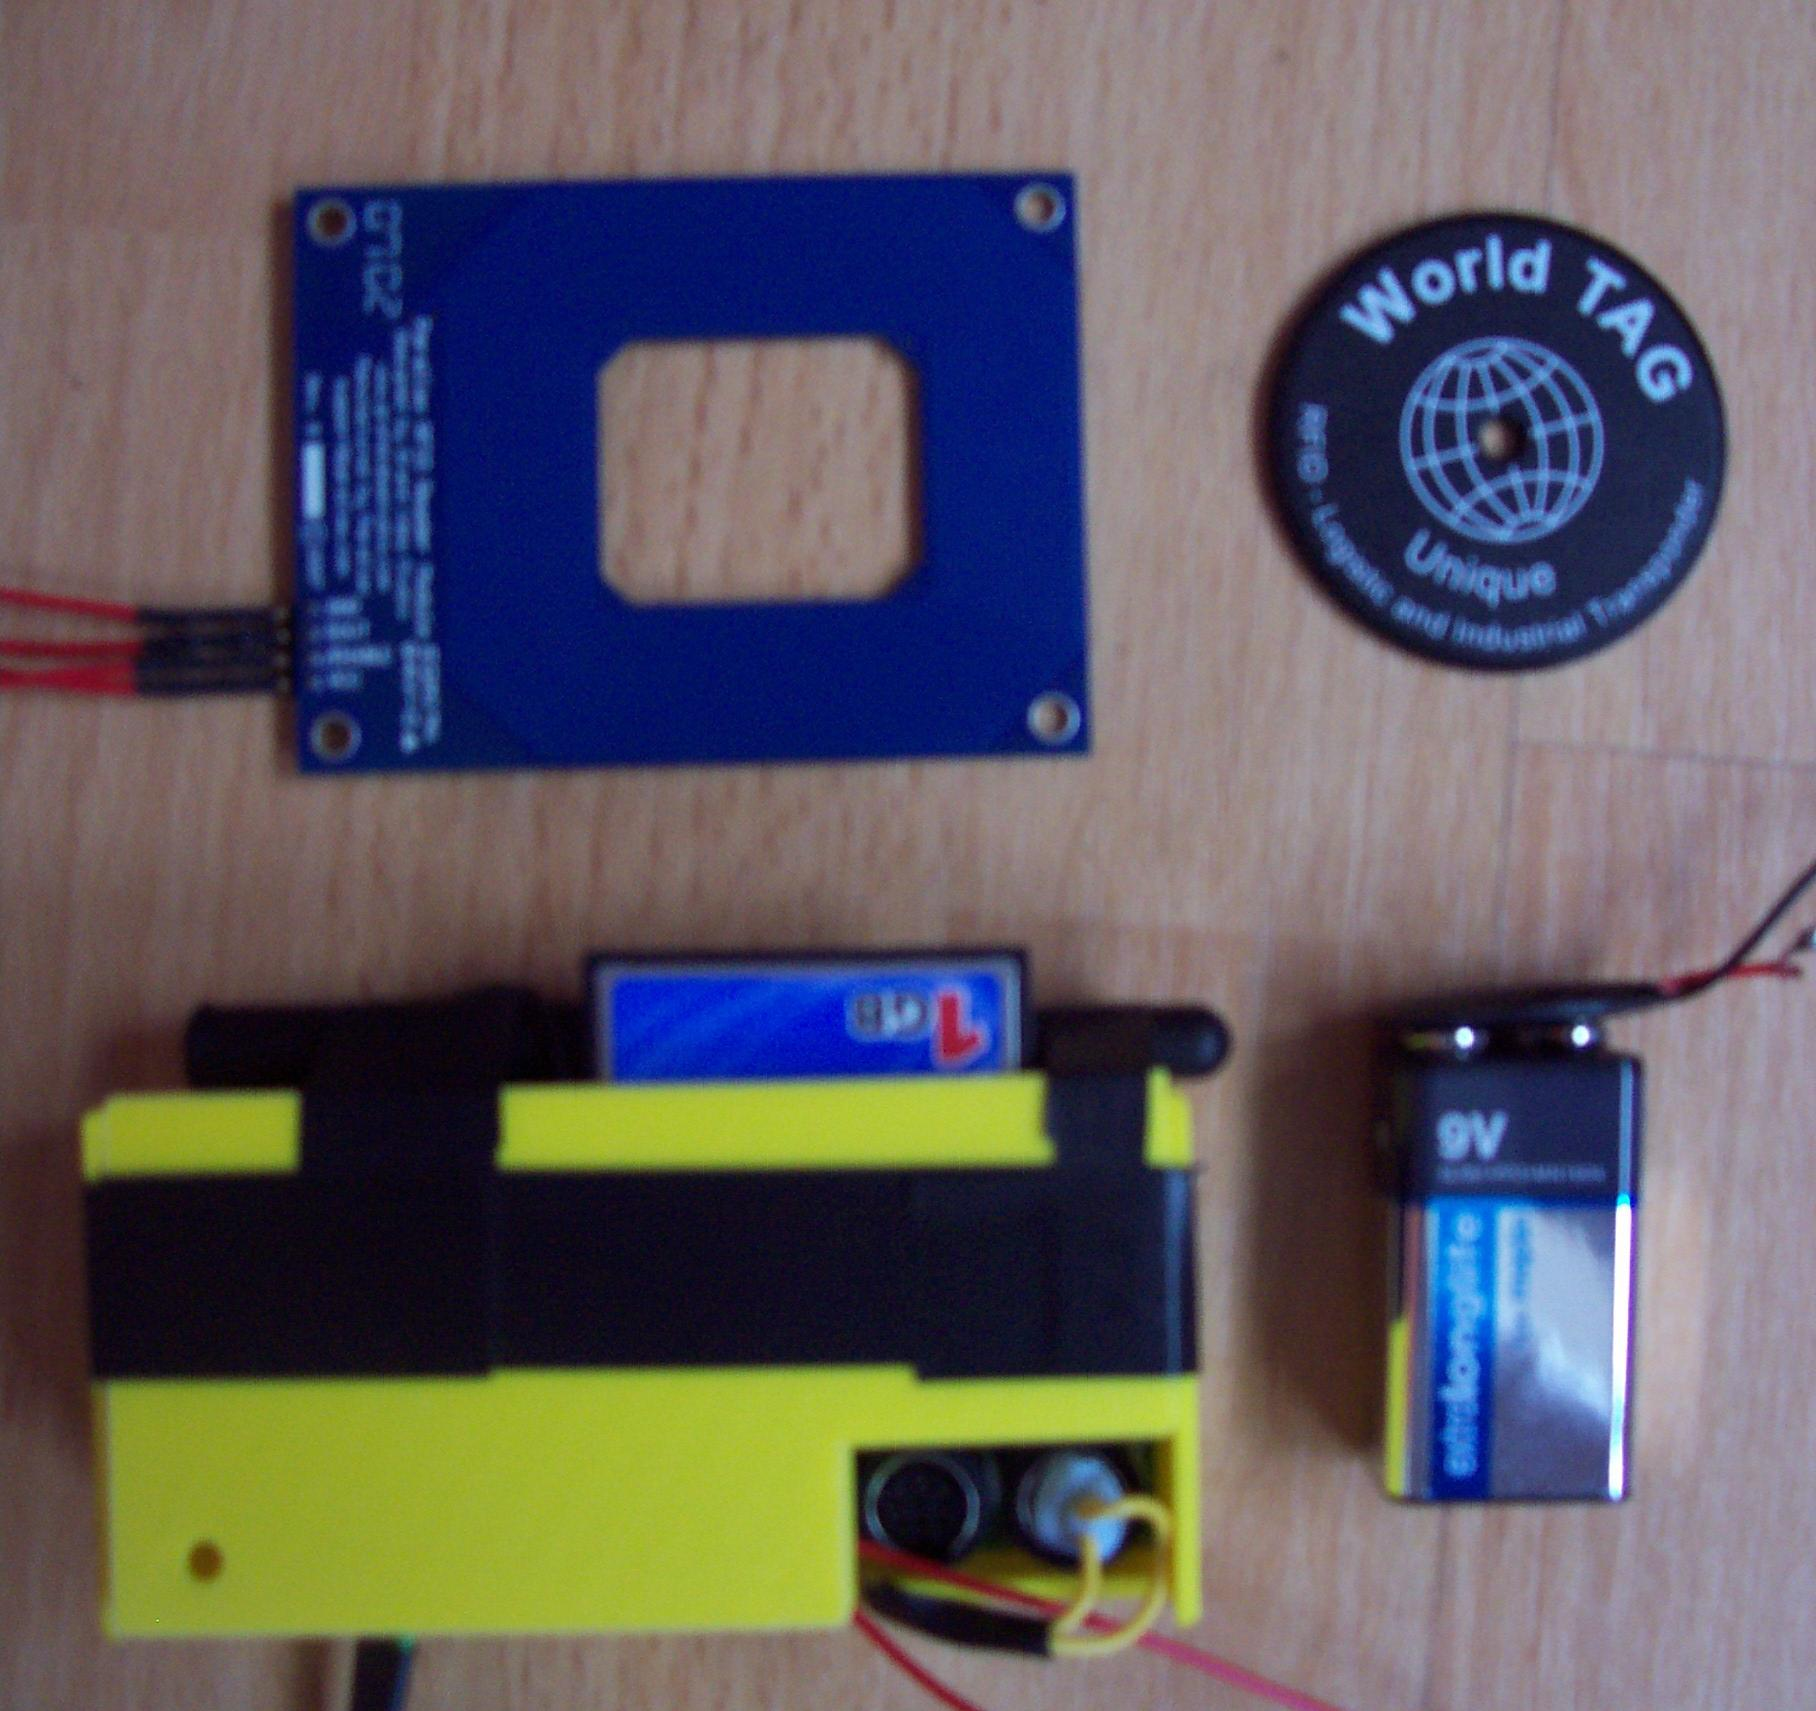
\includegraphics[width=6cm, height=6cm]{mobileShot}
}
\caption{RFID reader connected to Gumstix}
\label{fig:circuit}
\end{figure} 

Once a tag ID has been read and received by the Gumstix it is transmitted wirelessly to a server and stored in a database. The function of the server is to process tag read data and present it in an online lost and found system. The server runs on a laptop connected to a router which has been configured to allow port forwarding to the static IP address of the laptop. This means the Gumstix can be configured to connect to the router and use it as a bridge to transmit data to the server.  

A Bluetooth module is integrated into the Gumstix which is used to gather information about a users' interactions with other people and specific locations they have visited, such as home and college. People are identified based on their mobile phone Bluetooth ID. Locations can be identified using static Bluetooth nodes. Nodes consist of static computers with Bluetooth capabilities, where their unique ID corresponds to the specific location. When the Gumstix scans and identifies a Bluetooth ID it is transmitted wirelessly to the server and database in the same manner as RFID tag reads.  

\begin{figure}[h]
\centering
\fboxsep 2mm
\framebox{
	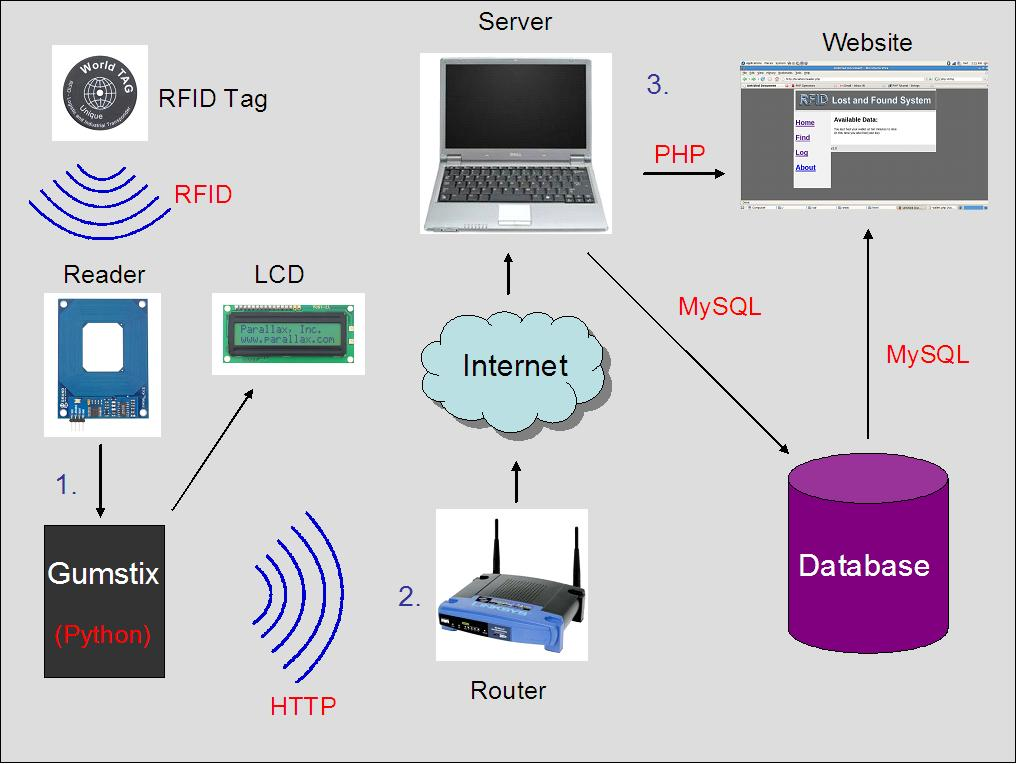
\includegraphics[width=14cm, height=9cm]{architecture}
}
\caption{System Architecture [Note: will be updated later to include LCD and Bluetooth]}
\label{fig:architecture}
\end{figure} 

\section{Data Processing}
The server setup used in this project is known as LAMP. The LAMP server system consists of a number of open source software technologies which are commonly used together in server applications. It consists of an Apache server~\footnote{Apache website: http://www.apache.org/}, MySQL~\footnote{MySQL website: www.mysql.com} for managing databases, and PHP~\footnote{PHP website: http://www.php.net/} scripting language used for server side data processing in dynamic web pages. These technologies are running on a Linux operating system. In this system the server hosts the webpages which are written using PHP. PHP allows interaction with the MySQL database, such as storing and retrieving data, and processes this information displaying it to the user through the website.

When the Gumstix is powered and boots up, it runs a Python script and C program. The C program connects to the serial port and reads in data from the RFID reader. The Python script is responsible for transmitting tag IDs to the server. When a tagged object is read by the RFID reader, its ID is passed through the serial port and passed to the Python script which interacts with a PHP page running on the server. When a tag is read, its ID is transmitted wirelessly via the router to the PHP page takes in the tag ID as a GET variable. This ID is stored in a database using MySQL queries embedded within the PHP page. Each ID is given a time stamp when it is stored, consisting of the current time and date, and is checked against a second database. The second database stores all tag ID's recognised by the system and what item the ID corresponds to. When a tag ID is stored this information is used to determine which item the ID corresponds to.

[insert data flow diagram, figure out how to do it first]

When a tag ID is read and transmitted to the database, the Python script will begin to gather more information using Bluetooth. It scans for devices and takes in any Bluetooth IDs within range. Using the same technique for processing tag reads, the Bluetooth IDs are transmitted and stored in the server database. Stored data consists of the Bluetooth ID, a time stamp, and if possible a name corresponding to the Bluetooth ID. For example, each Bluetooth ID read is checked against a table containing recognised IDs. These recognised IDs consist of known IDs, corresponding to locations and individual people. [Note: not yet decided if all bluetooth ids will be stored or only recognised ones???? :-/ ] 

\begin{figure}[h]
\centering
\fboxsep 2mm
\framebox{
	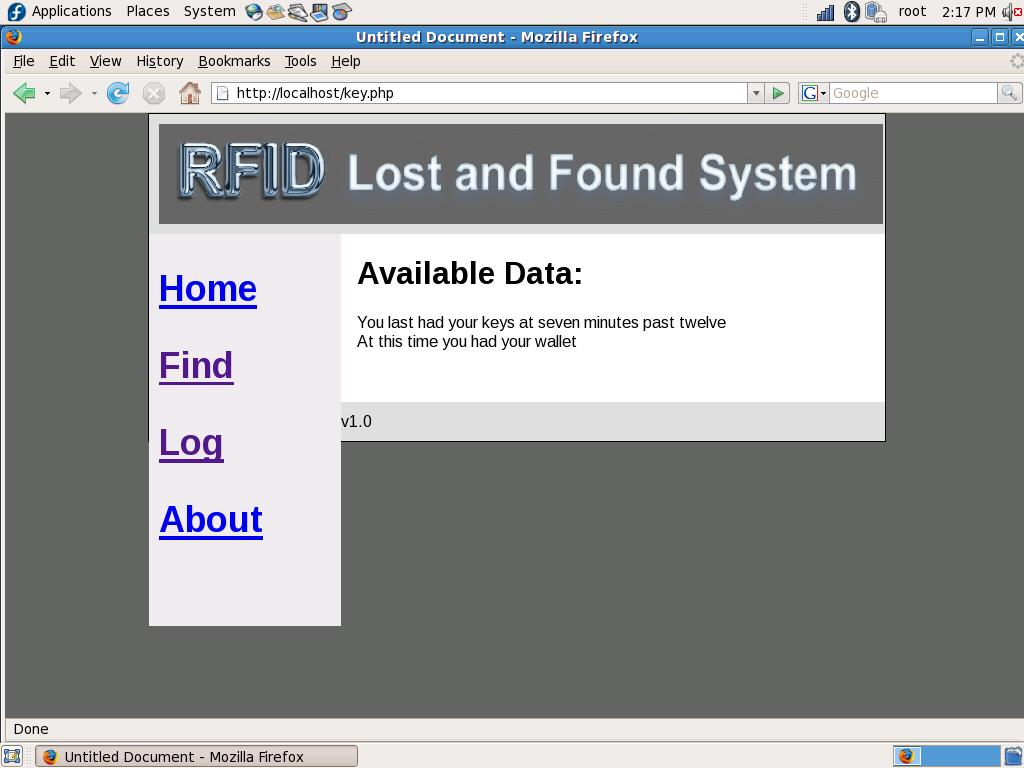
\includegraphics[width=13cm, height=8cm]{websiteShot}
}
\caption{Lost and Found website [Note: will be updated]}
\label{fig:webshot}
\end{figure} 

With RFID and Bluetooth data stored, a PHP website can incorporate this as part of the lost and found application. When a user loses an item they simply logon to this website and select the item they are looking for. Using PHP with MySQL the website can retrieve relevant information from the database. This data is presented to the user aiding them in remembering when and where they last had the item. One of the goals for this system is to return this information in the form of human readable cues, or in such a way that is as close as possible to human readable language. For example, You last had your wallet at two o clock. At this time you were at college and also interacting with your keys�. This is achieved within the PHP pages, formatting and filtering data, and displaying relevant information in the form of the human readable cues. The aim of using human readable cues is to create an application which people can easily relate to. It is the opinion of this author that a person can better relate to natural human language rather than lists of data consisting of dates, times and IDs. This however may not always be true and to explore each technique, the lost and found application can present data in both forms. The effectiveness of each technique is discussed in chapter~\ref{evaluations}. Figure \ref{fig:webshot} shows a screen shot from the web site.
    
\begin{itemize}
	\item Next paragraph will be about the LCD screen once i know how im doing it
\end{itemize}
\newpage

\chapter{System Testing and Evaluation}
\label{evaluations}

\section{System Evaluation}

\subsection{RFID Prototype}
Early system testing began with a working prototype implementing the RFID component. This consisted of the RFID reader connected to the Gumstix, setup of the LAMP server, and implementation of a simple lost and found website. This prototype was designed to evaluate a number of key components of the system. The circuit built for relaying tag ID's to the Gumstix serial port included an LED, which was used to indicate when tags were being read successfully. To ensure tag read data was being transferred successfully to the server, initially a simple test page was setup, which retrieved the contents of the database and displayed it on screen. Testing began by placing different tags at various ranges to the reader. The goal of this was to determine if tagged items could be successfully identified and their IDs transmitted and stored accurately. This testing also explored the limitations of the readers range. 

This evaluation produced some useful insight. The reader was found to have a very limited range of about three inches. However once a tag is within this range it is accurately identified. Viewing the test page, which displayed the contents of the database, indicated that once an ID is read, it is always transmitted and stored correctly in the database. This indicates that the hardware setup and data processing techniques are sound, however the readers range needed to be considered.   

\subsection{System Form Factor}
The goal of the systems form factor is to create a system which is small, compact and easily carried by the user. The second factor in its design was the address the issue of the readers range. A small pouch design can be placed within a pocket or bag along with other items. Due to the relatively small space of pockets and bags, items will be in close proximity to each other at all times. This aim of this test was to determine if this can overcome the readers limitations. 

Although the system is very compact and portable it is necessary to highlight that it is a proof of concept. If such a system was designed and built commercially it would be considerably smaller. For example the Gumstix computer is much more powerful than is necessary for the data processing involved in the system. 

\begin{itemize}
	\item Need to elaborate more on this, talk about printed circuits? Maybe i should'nt discuss this here maybe in implementation??
\end{itemize}
\begin{itemize}
	\item Talk about form factors effectiveness at reading tags when placed inside a bag and pocket. Need to make pouch!! Then test it by placing it in stuff with tagged items and see if it reads them successfully.
\end{itemize}

\subsection{Human Readable Cues}
To evaluate the human readable cues a survey was created to gather feedback on which technique people consider more effective, the human readable cues or raw data consisting of date and time stamps. 

\begin{itemize}
	\item Put survey here once its complete
\end{itemize}
\begin{itemize}
	\item Discuss the answers people gave
\end{itemize}

\subsection{Full System Evaluation}
\begin{itemize}
	\item Proof of concept demo, perhaps a mock scenario, will decide exactly what it is when implementation is complete
\end{itemize}

\section{Results}
\label{testresults}

\newpage

\chapter{Conclusions and Future Work}
\label{future}

\section{Conclusions}
The primary goal of this project was to design a memory aid system using RFID technology and to determine its effectiveness in this task. An important component of the system was the ability to identify objects. The initial system prototype was a basic version of the system which was designed to test the effectiveness of RFID technology for identifying items. The RFID reader was found to be accurate at identifying tagged objects which suggests that it is a useful and effective technology for implementing such a system. While the effectiveness of reading tags was found to be very accurate the reader did have a limited range. This influenced the systems form factor and how the system was used. 

\begin{itemize}
	\item Talk more about form factor, did it work?
\end{itemize}
\begin{itemize}
	\item Im finding this section hard, i think it will come to me closer to completion ;-)
\end{itemize}
   

\section{Future Work}
\begin{itemize}
	\item What did/ didnt work? How might it be improved?
\end{itemize}
\begin{itemize}
	\item If bluetooth does'nt work out in the end talk about it here.
\end{itemize}
\begin{itemize}
	\item The LCD screen will be fairly simple, maybe think of ways it could be more useful and suggest how it could be done
\end{itemize}
\begin{itemize}
	\item Discuss Fintans ideas. Will be leaving this till the very end
\end{itemize}

\newpage

%%%% ADD YOUR BIBLIOGRAPHY HERE
\newpage\label{endpage}
\bibliography{ref}
\end{document}

\end{article}
